\documentclass[a4paper, 12pt, final, garamond]{book}
\usepackage{cours-preambule}

\raggedbottom

\makeatletter
\renewcommand{\@chapapp}{Optique -- chapitre}
\makeatother

\begin{document}
\setcounter{chapter}{2}

\chapter{TD~: Miroir plan et lentilles minces}

\section{Constructions optiques de lentilles}

Construisez les images par la lentille des objets suivants. On donnera à chaque
fois la nature de l'objet et de l'image.

\subsection{Pour une lentille convergente}
\begin{enumerate}
    \item Objet avant le foyer objet~;
    \item Objet sur le foyer objet~;
    \item Objet entre le foyer objet et la lentille~;
    \item Objet après la lentille~;
    \item Faisceau parallèle à l'axe optique~;
    \item Rayon quelconque incliné par rapport à l'axe optique.
\end{enumerate}

\subsection{Pour une lentille divergente}
\begin{enumerate}
    \item Objet avant le foyer image~;
    \item Objet entre le foyer objet et la lentille~;
    \item Objet sur le foyer objet~;
    \item Objet après le foyer objet~;
    \item Faisceau parallèle à l'axe optique~;
    \item Rayon quelconque incliné par rapport à l'axe optique.
\end{enumerate}

\section{Constructions optiques de miroirs}
Dans chacune des situations suivantes, déterminer la nature des faisceaux,
nommer les intersections dessinées, compléter la marche des rayons lumineux et
commenter la nature de l'objet et de l'image.
\begin{center}
    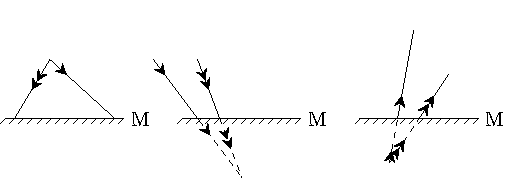
\includegraphics[height=4cm]{miroir_plan.pdf}
\end{center}

\section{Vidéoprojecteur}

On modélise l'objectif d'un vidéoprojecteur par une lentille mince convergente
de distance focale de \SI{5.0}{cm}. L'objet transverse a une hauteur de
\SI{24}{mm} et l'écran se situe à \SI{4.0}{m} de la lentille. Déterminer la
position, la nature de l'objet ainsi que la taille de l'image.

\section{Œil réduit et accommodation}
Le cristallin de l'œil est assimilable à une lentille mince de distance focale
variable (accommodation). L'image, pour être nette, doit se former sur la rétine
qui est située à \SI{22.3}{mm} du cristallin. Lorsque l'œil n'accommode pas
(cristallin au repos), il voit nettement un objet situé à l'infini. Lorsqu'il
accommode au maximum, il voit nettement un objet jusqu'à \SI{25}{cm} (valeur
moyenne).
\begin{enumerate}
    \item Quelles sont la vergence et la distance focale du cristallin lorsque
        l'œil voit nettement un objet placé à \SI{25}{cm}~? À l'infini~?
    \item On observe nettement un objet de \SI{10}{cm} de haut placé à
        \SI{1}{m}. Quelle est la vergence du cristallin~?
    \item Dans ces conditions d'observation, quels sont le sens et la taille de
        l'image formée sur la rétine~?
\end{enumerate}

\section{Coin de miroir}
Un rayon lumineux pénètre dans un système optique composé de deux miroirs plans
faisant un angle $\alpha$ entre eux. Il rentre parallèlement à un
miroir et ressort du système en revenant sur lui-même par le même chemin
optique après trois réflexions. Quelle est la valeur de $\alpha$~?

\section{Étude d'un rétroprojecteur}
\begin{wrapfigure}[10]{R}{.4\linewidth}
    \vspace*{-20pt}
    \centering
    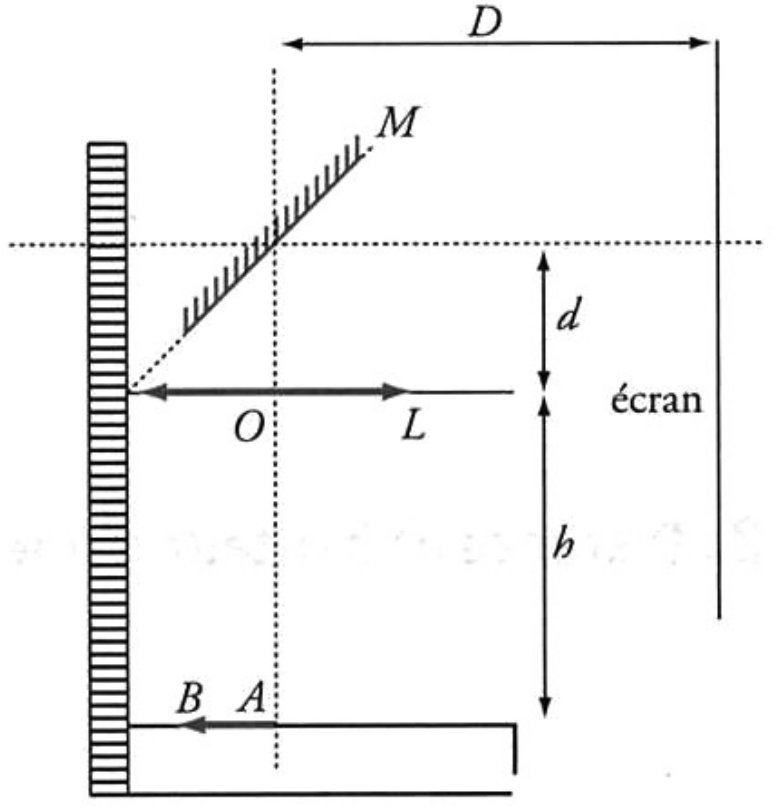
\includegraphics[width=\linewidth]{retro}
    \caption{Schéma du rétroprojecteur}
    \label{fig:retro}
\end{wrapfigure}

Un rétroprojecteur est un ensemble lentille-miroir, avec un miroir plan incliné
à \ang{45;;} par rapport à la lentille. L'ensemble lentille-miroir est réglable
en hauteur ($h$). On étudie un rétroprojecteur dont la lentille a une vergence
de $\SI{2.0}{\delta}$, avec une distance lentille-miroir $d = \SI{10}{cm}$. 

On désire projeter un objet transparent $AB$ sur un écran placé à $D =
\SI{3.0}{m}$ de l'axe optique de la lentille.

\begin{enumerate}
    \item Déterminer la distance $h$ permettant d'obtenir une image nette sur
        l'écran.
    \item Calculer le grandissement.
\end{enumerate}

\end{document}
